\documentclass{article}
\usepackage{fourier}
\usepackage{fullpage}
\usepackage{graphicx}
\usepackage{xspace}
\usepackage{epigraph}
\usepackage{listings}
\usepackage{xcolor}
\usepackage{url}
\usepackage{soul}
\usepackage{multirow}
\usepackage{clrscode3e}
\usepackage{hyperref}
\usepackage{wrapfig}
\usepackage{amsmath}
\usepackage{tikz}
\usetikzlibrary{calc,shapes.multipart,chains,arrows}

\title{Assignment 6\\The Great Firewall of Santa Cruz:\\Bloom Filters,
Linked Lists and Hash Tables}
\author{Prof. Darrell Long \\
CSE 13S -- Winter 2021}
\date{Due: February $28^\text{th}$ at 11:59 pm PST}

\usepackage{fancyhdr}
\pagestyle{fancy}
\fancyhf{}

\fancypagestyle{plain}{%
  \fancyhf{}
  \renewcommand{\headrulewidth}{0pt}
  \renewcommand{\footrulewidth}{0pt}
  \lfoot{\textcopyright{} 2021 Darrell Long}
  \rfoot{\thepage}
}

\pagestyle{plain}

\definecolor{codegreen}{rgb}{0,0.5,0}
\definecolor{codegray}{rgb}{0.5,0.5,0.5}
\definecolor{codepurple}{rgb}{0.58,0,0.82}

\lstloadlanguages{C,make,python,fortran,bash}

\lstdefinestyle{bashstyle}{
  language=bash,
  basicstyle=\small\ttfamily,
  numbers=none,
  frame=tb,
  columns=fullflexible,
  backgroundcolor=\color{yellow!10},
  linewidth=0.9\linewidth,
  xleftmargin=0.1\linewidth,
  aboveskip=1.25em,
  belowskip=1.25em,
  breakatwhitespace=false,
  breaklines=true,
  showstringspaces=false,
  keepspaces=true,
  showspaces=false,
  showtabs=false,
  tabsize=4
}

\lstdefinestyle{plainstyle}{
  keywords={},
  stringstyle=\color{black},
  basicstyle=\small\ttfamily,
  numbers=none,
  frame=tb,
  columns=fullflexible,
  backgroundcolor=\color{yellow!10},
  linewidth=0.9\linewidth,
  xleftmargin=0.1\linewidth,
  aboveskip=1.25em,
  belowskip=1.25em,
  breakatwhitespace=false,
  breaklines=true,
  showstringspaces=false,
  keepspaces=true,
  showspaces=false,
  showtabs=false,
  tabsize=4
}

\lstdefinestyle{c99}{
    language=C,
    morekeywords={
      bool, uint8_t, uint16_t, uint32_t, uint64_t,
      int8_t, int16_t, int32_t, int64_t
    },
    upquote=true,
    commentstyle=\color{codegreen},
    keywordstyle=\color{magenta},
    identifierstyle=\color{black},
    stringstyle=\color{codepurple},
    basicstyle=\ttfamily,
    breakatwhitespace=false,
    breaklines=true,
    captionpos=b,
    keepspaces=true,
    showspaces=false,
    showstringspaces=false,
    showtabs=false,
    numbers=left,
    numbersep=7pt,
    numberstyle=\ttfamily\color{black!25},
    xleftmargin=12pt,
    tabsize=4
}

\lstdefinestyle{python}{
    language=python,
    upquote=true,
    commentstyle=\color{codegreen},
    keywordstyle=\color{magenta},
    identifierstyle=\color{black},
    stringstyle=\color{codepurple},
    basicstyle=\ttfamily,
    breakatwhitespace=false,
    breaklines=true,
    captionpos=b,
    keepspaces=true,
    showspaces=false,
    showstringspaces=false,
    showtabs=false,
    numbers=left,
    numbersep=7pt,
    numberstyle=\ttfamily\color{black!25},
    xleftmargin=12pt,
    tabsize=4
}

\usepackage[most]{tcolorbox}

\newtcolorbox{prelab}[1]{
  colback=red!5!white, colframe=red!75!black, title=#1
}

\newtcblisting{codelisting}[2][]{
  title=#2, #1,
  fonttitle=\bfseries,
  colframe=black!80,
  listing only,
  listing options={basicstyle=\ttfamily,style=c99},
  top=-5pt,
  bottom=-5pt,
  enlarge top by=10pt
}

\newtcblisting{pythonlisting}[2][]{
  title=#2, #1,
  fonttitle=\bfseries,
  colframe=black!80,
  listing only,
  listing options={basicstyle=\ttfamily,style=python},
  top=-5pt,
  bottom=-5pt,
  enlarge top by=5pt
}

\newcommand\Warning{%
 \makebox[1.4em][c]{%
 \makebox[0pt][c]{\raisebox{.1em}{\small!}}%
 \makebox[0pt][c]{\color{red}\Large$\bigtriangleup$}}}%


\begin{document}\maketitle

\section{Introduction}

\epigraphwidth=0.5\textwidth \epigraph{\emph{War is peace. Freedom
is slavery. Ignorance is strength.}}{---George Orwell, 1984}

\noindent You have been selected through thoroughly democratic processes
(and the machinations of your friend and hero Ernst Blofeld) to be the
Dear and Beloved Leader of the Glorious People's Republic of Santa Cruz
following the failure of the short-lived anarcho-syndicalist commune,
where each person in turn acted as a form of executive officer for the
week. In order to promote virtue and prevent vice, and to preserve
social cohesion and discourage unrest, you have decided that the
Internet content must be filtered so that your beloved children are not
corrupted through the use of unfortunate, hurtful, offensive, and far
too descriptive language.


\section{Bloom Filters}

\epigraphwidth=0.75\textwidth
\epigraph{\emph{The Ministry of Peace concerns itself with war, the Ministry
of Truth with lies, the Ministry of Love with torture and the Ministry of
Plenty with starvation. These contradictions are not accidental, nor do they
result from from ordinary hypocrisy: they are deliberate exercises in
\textbf{doublethink}.}}{---George Orwell, 1984}

\begin{wrapfigure}{r}{0.133\textwidth}
\centering
\includegraphics[width=0.12\textwidth]{1984-Big-Brother.jpg}
\end{wrapfigure}

\noindent The Internet is very large, very fast, and full of
\emph{badthink}. The masses spend their days sending each other cat
videos and spewing \emph{oldspeak}---very bad indeed. You decide, as the
newly elected Dear and Beloved Leader of the Glorious People's Republic
of Santa Cruz (GPRSC), that a more neutral \emph{newspeak} is required
to keep the citizens of the GPRSC content, pure, and from thinking too
much. But how do you process and store so many words as they flow in and
out of the GPRSC at $10\,$Gbits/second? The solution comes to your
brilliant and pure mind---a \emph{Bloom filter}.

A Bloom filter is a space-efficient probabilistic data structure,
conceived by Burton H. Bloom in 1970, and is used to test whether
an element is a member of a set. False-positive matches are possible,
but false negatives are not---in other words, a query for set membership
returns either ``possibly in the set'' or ``definitely not in the set.''
Elements can be added to the set but not removed from it; the more
elements added, the higher the probability of false positives.

A Bloom filter can be represented as an array of $m$ bits, or a
\textbf{bit vector}. A Bloom filter should utilize $k$ different hash
functions. Using these hash functions, a set element added to the Bloom
filter is mapped to at most $k$ of the $m$ bit indices, generating a
uniform pseudo-random distribution. Typically, $k$ is a small constant
which depends on the desired false error rate $\epsilon$, while $m$ is
proportional to $k$ and the number of elements to be added.

Assume you are adding an word $w$ to your Bloom filter and are using
$k=3$ hash functions, $f(x)$, $g(x)$, and $h(x)$. To add $w$ to the
Bloom filter, you simply set the bits at indices $f(w)$, $g(w)$, and
$h(w)$. To check if some word $w'$ has been added to the same Bloom
filter, you check if the bits at indices $f(w')$, $g(w')$, and $h(w')$
are set. If they are all set, then $w'$ has \emph{most likely} been
added to the Bloom filter. If any one of those bits was cleared, then
$w'$ has definitely \emph{not} been added to the Bloom filter. The fact
that the Bloom filter can only tell if some word has \emph{most likely}
been added to the Bloom filter means that \emph{false positives} can
occur. The larger the Bloom filter, the lower the chances of getting
false positives.

So what do Bloom filters mean for you as the Dear and Beloved Leader?
It means you can take a list of proscribed words, \emph{oldspeak} and
add each word into your Bloom filter. If any of the words that your
citizens use seem to be added to the Bloom filter, then this is very
ungood and further action must be taken to discern whether or not the
citizen did transgress. You decide to implement a Bloom filter with
\emph{three} salts for \emph{three} different
hash functions. Why? To reduce the chance of a \emph{false positive}.

You can think of a ``salt'' as an initialization vector or a key.
Using different salts with the same hash function results in a
different, unique hash. Since you are equipping your Bloom filter with
three different salts, you are effectively getting three different hash
functions: $f(x)$, $g(x)$, and $h(x)$. Hashing a word $w$, with
extremely high probability, should result in $f(w) \ne g(w) \ne h(w)$.
These salts are to be used for the SPECK cipher, which requires a
128-bit key, so we have used MD5 \footnote{Rivest, R.. “The MD5
Message-Digest Algorithm.” RFC 1321 (1992): 1-21.} ``message-digest'' to
reduce three books down to 128 bits each. You will use the SPECK cipher
as a hash function, which will be explained in \S 5.1,

\subsection{\texttt{BloomFilter}}

The following \texttt{struct} defines the \texttt{BloomFilter} ADT. The
three salts will be stored in the \texttt{primary}, \texttt{secondary},
and \texttt{tertiary} fields. Each salt is 128 bits in size. To hold
these 128 bits, we use an array of two \texttt{uint64\_t}s. This
\texttt{struct} definition \emph{must} go in \texttt{bf.c}.

\begin{codelisting}{}
struct BloomFilter {
  uint64_t primary[2];   // Primary hash function salt.
  uint64_t secondary[2]; // Secondary hash function salt.
  uint64_t tertiary[2];  // Tertiary hash function salt.
  BitVector *filter;
};
\end{codelisting}

\subsection{\texttt{BloomFilter *bf\_create(uint32\_t size)}}

The constructor for a Bloom filter. Working code for the constructor,
complete with primary, secondary, and tertiary salts that you will use,
is shown below. Note that you will also have to implement the bit vector
ADT for your Bloom filter, as it will serve as the array of bits
necessary for a proper Bloom filter.

\begin{codelisting}{}
BloomFilter *bf_create(uint32_t size) {
  BloomFilter *bf = (BloomFilter *) malloc(sizeof(BloomFilter));
  if (bf) {
    // Fear & Loathing in Las Vegas
    bf->primary[0] = 0x02d232593fbe42ff;
    bf->primary[1] = 0x3775cfbf0794f152;
    // A Moveable Feast
    bf->secondary[0] = 0xc1706bc17ececc04;
    bf->secondary[1] = 0xe9820aa4d2b8261a;
    // The Cremation of Sam McGee
    bf->tertiary[0] = 0xd37b01df0ae8f8d0;
    bf->tertiary[1] = 0x911d454886ca7cf7;
    bf->filter = bv_create(size);
    if (!bf->filter) {
      free(bf);
      bf = NULL;
    }
  }
  return bf;
}
\end{codelisting}

\subsection{\texttt{void bf\_delete(BloomFilter **bf)}}

The destructor for a Bloom filter. As with all other destructors, it
should free any memory allocated by the constructor and null out the
pointer that was passed in.

\subsection{\texttt{uint32\_t bf\_size(BloomFilter *bf)}}

Returns the size of the Bloom filter. In other words, the number of bits
that the Bloom filter can access. Hint: this is the length of the
underlying bit vector.

\subsection{\texttt{void bf\_insert(BloomFilter *bf, char *oldspeak)}}

Takes \texttt{oldspeak} and inserts it into the Bloom filter. This
entails hashing \texttt{oldspeak} with each of the three salts for three
indices, and setting the bits at those indices in the underlying bit
vector.

\subsection{\texttt{bool bf\_probe(BloomFilter *bf, char *oldspeak)}}

Probes the Bloom filter for \texttt{oldspeak}. Like with
\texttt{bf\_insert()}, \texttt{oldspeak} is hashed with each of the
three salts for three indices. If all the bits at those indices are set,
return \texttt{true} to signify that \texttt{oldspeak} was most likely
added to the Bloom filter. Else, return \texttt{false}.

\subsection{\texttt{void bf\_print(BloomFilter *bf)}}

A debug function to print out a Bloom filter.

\vspace{10pt}
\begin{prelab}{Pre-lab Part 1}
  \begin{enumerate}
    \item Write down the pseudocode for inserting and deleting elements from a
        Bloom filter.
  \end{enumerate}
\end{prelab}


\section{Bit Vectors}

\epigraph{\emph{Symmetrical equations are good in their place, but `vector'
is a useless survival, or offshoot from quaternions, and has never been of the
slightest use to any creature.}}{---Lord Kelvin}

\noindent \textit{\textbf{Bit vectors}} are a rarely taught but
essential tool in the kit of all computer scientists and engineers. A
bit vector is an ADT that represents an array of bits, the bits in which
are used to denote if something is true or false (1 or 0). This is an
efficient ADT since, in order to represent the truth or falsity of an
array of $n$ items, we can use $n / 8$ if $n \equiv 0 \pmod 8$ else
$\lfloor n / 8 \rfloor + 1$ \texttt{uint8\_t}'s instead of $n$, and
being able to access $8$ indices with a single integer access is
extremely cost efficient.

\begin{codelisting}{}
struct BitVector {
  uint32_t length;
  uint8_t *vector;
};
\end{codelisting}

You must implement each of the functions specified in the header file. Most of
them are just a line of two of \textbf{C} code, but their implementation can be
subtle. Since, you have already implemented a bit matrix, you will find
that their implementations are similar. You are warned \emph{again}
against using code that you may find on the Internet.

\subsection{\texttt{BitVector *bv\_create(uint32\_t length)}}

This constructor will allocate memory for the bit vector.  The number of
bits that \texttt{vector} should hold is \texttt{length}.  If at any
point allocating memory with \texttt{calloc()} fails, the function must
return \texttt{NULL}, else it must return a \texttt{BitVector *} or a
pointer to a \texttt{BitVector}.

\subsection{\texttt{void bv\_delete(BitVector **bv)}}

The destructor will free the memory allocated for the bit vector. This
requires freeing memory for the array, \texttt{vector}, followed by
freeing the structure itself. It is best practice to set a pointer to
\texttt{NULL} once it has been freed to avoid dereferencing a
\texttt{NULL} pointer in the future (in reality you should check if a
pointer is valid before dereferencing it). In order to set \texttt{bv}
to \texttt{NULL}, we need the address of the pointer to the
bit vector, hence the reason for a double pointer as a parameter.

\subsection{\texttt{uint32\_t bv\_length(BitVector *bv)}}

Returns the bit vector's length.

\subsection{\texttt{void bv\_set\_bit(BitVector *bv, uint32\_t i)}}

Upon creation, the elements of a bit vector will be initialized to 0.
Since we cannot directly access a bit in a \texttt{uint8\_t}, we instead
need to perform bitwise operations on bytes in order to set a specific
bit. The location of the byte where the bit in question, \texttt{i},
resides is given by the following:
\texttt{vector[$\lfloor$i$/8\rfloor$]}. Then a bitwise operation is
needed to set the correct bit, \texttt{i}. Setting a bit should not
interfere with any of the other bits' values.

\subsection{\texttt{void bv\_clr\_bit(BitVector *bv, uint32\_t i)}}

In some cases it may be necessary to clear a bit or element in a
bit vector. Similarly to setting a bit, it is necessary to access the
byte where the bit specified by \texttt{i} is located. The location of
the byte is given by the following:
\texttt{vector[$\lfloor$i$/8\rfloor$]}.  Then bitwise operations are
needed to clear the correct bit, \texttt{i}.  Clearing a bit should not
interfere with any of the other bits' values.

\subsection{\texttt{uint8\_t bv\_get\_bit(BitVector *bv, uint32\_t i)}}

As mentioned in \S 3, it is necessary to be able to get specific bits
from the Bloom filter to determine if one of your dear citizens has used
improper oldspeak. Thus, we need a function get a bit from a bit
vector.  Just like setting and clearing a bit, we need to access the
$\lfloor i/8 \rfloor^\text{th}$ byte in \texttt{vector} to retrieve the value
of the $i^{th}$ bit. Then bitwise operations are needed to get the value
of the bit. This function should return a 1 if the bit is set and 0
otherwise.

\subsection{\texttt{void bv\_print(BitVector *bv)}}

For debugging purposes it is helpful to print out a bit vector.
\textcolor{red}{\emph{Do this first.}}


\section{Hash Tables}

\epigraph{\emph{To send men to the firing squad, judicial proof is
unnecessary \ldots These procedures are an archaic bourgeois
detail.}}{Ernesto Ch\'e Guevara}

\noindent Armed with a Bloom filter, you now exercise the power to catch and
punish those who practice wrongthink and continue to use oldspeak. It
comes to mind however, that a Bloom filter is probabilistic and that it
is better to exercise mercy and counsel the oldspeakers so that they may
atone and use \emph{newspeak}. To remedy this, another solution pops
into your brilliant and pure mind---a \emph{hash table}.

A hash table is a data structure that maps keys to values and provides
fast, $\operatorname{O}(1)$, look-up times. It does so typically by
taking a key $k$, hashing it with some hash function $h(x)$, and placing
the key's corresponding value in an underlying array at index $h(k)$.
This is the perfect way not only to store translations from oldspeak to
newspeak, but also as a way to store all prohibited oldspeak words
without newspeak translations. We will refer to oldspeak without
newspeak translations as \emph{badspeak}. So what happens when two
\emph{oldspeak} words have the same hash value?  This is called a
\emph{hash collision}, and must be resolved. Rather than doing
\emph{open addressing} (as will be discussed in lecture), we will be
using \emph{linked lists} to resolve \emph{oldspeak} hash collisions.
First, however, we must discuss the hash function.

\begin{wrapfigure}{r}{0.133\textwidth}
\centering
\includegraphics[width=0.130\textwidth]{Blofeld.png}
\end{wrapfigure}

\subsection{Hashing with the SPECK Cipher}

You will need a good hash function to use in your Bloom filter and hash
table. We will have discussed hash functions in class, and rather than
risk having a poor one implemented, we will simply provide you one. The
SPECK\footnote{ Ray Beaulieu, Stefan Treatman-Clark, Douglas Shors,
  Bryan Weeks, Jason Smith, and Louis Wingers, ``The {SIMON} and {SPECK}
lightweight block ciphers.'' In Proceedings of the 52nd ACM/EDAC/IEEE
Design Automation Conference (DAC), pp.  1--6. IEEE, 2015.} block cipher
is provided for use as a hash function.

SPECK is a family of lightweight block ciphers publicly released by the
National Security Agency (NSA) in June 2013.  SPECK has been optimized
for performance in software implementations, while its sister algorithm,
SIMON, has been optimized for hardware implementations. SPECK is an
add-rotate-xor (ARX) cipher. The reason a cipher is used for this is
because encryption generates random output given some input; exactly
what we want for a hash.

Encryption is the process of taking some file you wish to protect,
usually called plaintext, and transforming its data such that only
authorized parties can access it. This transformed data is referred to
as ciphertext. Decryption is the inverse operation of encryption, taking
the ciphertext and transforming the encrypted data back to its original
state as found in the original plaintext. Encryption algorithms that
utilize the same key for both encryption and decryption, like SPECK, are
symmetric-key algorithms, and algorithms that don't, such as RSA, are
asymmetric-key algorithms.

You will be given two files, \texttt{speck.h} and \texttt{speck.c}. The
former will provide the interface to using the SPECK hash function which
has been named \texttt{hash()}, and the latter contains the
implementation. The hash function \texttt{hash()} takes two parameters:
a 128-bit salt passed in the form of an array of two
\texttt{uint64\_t}s, and a key to hash. The function will return a
\texttt{uint32\_t} which is exactly the index the key is mapped to.

\begin{codelisting}{}
uint32_t hash(uint64_t salt[], char *key);
\end{codelisting}{}

\subsection{\texttt{HashTable}}

Below is the \texttt{struct} definition for a hash table. Similar to a
Bloom filter, a hash table contains a salt which is passed to
\texttt{hash()} whenever a new oldspeak entry is being inserted. As
mentioned in \S 5, we will be using linked lists to resolve oldspeak
hash collisions, which is why a hash table contains an array of linked
lists. The \texttt{mtf} field indicates whether or not the linked
lists should use the \emph{move-to-front} technique, which will be
discussed in \S 5.6.

\begin{codelisting}{}
struct HashTable {
  uint64_t salt[2];
  uint32_t size;
  bool mtf;
  LinkedList **lists;
};
\end{codelisting}

\subsection{\texttt{HashTable *ht\_create(uint32\_t size, bool mtf)}}

The constructor for a hash table. The \texttt{size} parameter denotes
the number of indices, or linked lists, that the hash table can index up
to. The salt for the hash table has been supplied in the constructor as
well.

\begin{codelisting}{}
HashTable *ht_create(uint32_t size, bool mtf) {
  HashTable *ht = (HashTable *) malloc(sizeof(HashTable));
  if (ht) {
    ht->salt[0] = 0x85ae998311115ae3; // Il nome della rosa
    ht->salt[1] = 0xb6fac2ae33a40089;
    ht->size = size;
    ht->mtf = mtf;
    ht->lists = (LinkedList **) calloc(size, sizeof(LinkedList *));
    if (!ht->lists) {
      free(ht);
      ht = NULL;
    }
  }
  return ht;
}
\end{codelisting}

\subsection{\texttt{void ht\_delete(HashTable **ht)}}

The destructor for a hash table. Each of the linked lists in
\texttt{lists}, the underlying array of linked lists, is freed.
The pointer that was passed in should be set to \texttt{NULL}.

\subsection{\texttt{uint32\_t ht\_size(HashTable *ht)}}

Returns the hash table's size.

\subsection{\texttt{Node *ht\_lookup(HashTable *ht, char *oldspeak)}}

Searches for an entry, a node, in the hash table that contains
\texttt{oldspeak}. A node stores oldspeak and its newspeak translation.
The index of the linked list to perform a look-up on is calculated by
hashing the \texttt{oldspeak}. If the node is found, the pointer to the
node is returned. Else, a \texttt{NULL} pointer is returned.

\subsection{\texttt{void ht\_insert(HashTable *ht, char *oldspeak,
char *newspeak)}}

Inserts the specified \texttt{oldspeak} and its corresponding
\texttt{newspeak} translation into the hash table. The index of the
linked list to insert into is calculated by hashing the
\texttt{oldspeak}. If the linked list that should be inserted into
hasn't been initialized yet, create it first before inserting the
oldspeak and newspeak.

\subsection{\texttt{void ht\_print(HashTable *ht)}}

A debug function to print out the contents of a hash table.

\section{Linked Lists}

\epigraph{\emph{Education is a weapon, whose effect depends on who holds
it in his hands and at whom it is aimed.}}{---Joseph Stalin}

\noindent A \emph{linked list} will be used to resolve hash collisions.
Each node of the linked list contains \emph{oldspeak} and its
\emph{newspeak} translation if it exists. The \emph{key} to search with
in the linked list is \emph{oldspeak}. Each node will also contain a
pointer to the previous node \emph{and} the next node in the linked
list. This is because you will be implementing \emph{doubly linked
lists}.

\subsection{\texttt{Node}}

A node is defined with the following \texttt{struct}:

\begin{codelisting}{}
struct Node {
  char *oldspeak;
  char *newspeak;
  Node *next;
  Node *prev;
};
\end{codelisting}

If the \texttt{newspeak} field is \texttt{NULL}, then the oldspeak
contained in this node is badspeak, since there is no newspeak
translation. This \texttt{struct} definition and interface for the node
ADT will be provided for you in \texttt{node.h}. The node ADT is not
opaque in order to simplify the rest of the linked list implementation.

\subsection{\texttt{Node *node\_create(char *oldspeak, char *newspeak)}}

The constructor for a node. You will want to make a \emph{copy} of the
\texttt{oldspeak} and its \texttt{newspeak} translation that are passed
in. What this means is \emph{allocating memory} and copying over the
characters for both \texttt{oldspeak} and \texttt{newspeak}. There was a
function \texttt{strdup()} that did precisely that, but it has been
deprecated. You will find it helpful to implement your own function to
mimic \texttt{strdup()}.

\subsection{\texttt{void node\_delete(Node **n)}}

The destructor for a node. Only the node \texttt{n} is freed. The
previous and next nodes that \texttt{n} points to \emph{are not}
deleted. Since you have allocated memory for \texttt{oldspeak} and
\texttt{newspeak}, remember to free the memory allocated to both of
those as well. The pointer to the node should be set to \texttt{NULL}.

\subsection{\texttt{void node\_print(Node *n)}}

While helpful as debug function, you will use this function to produce
correct program output. Thus, it is imperative that you print out the
contents of a node in the following manner:

\begin{itemize}
  \item If the node \texttt{n} contains oldspeak \emph{and} newspeak,
    print out the node with this print statement:
    \begin{codelisting}{}
printf("%s -> %s\n", n->oldspeak, n->newspeak);
    \end{codelisting}
  \item If the node \texttt{n} contains \emph{only} oldspeak, meaning
    that newspeak is null, then print out the node with this print
    statement:
    \begin{codelisting}{}
printf("%s\n", n->oldspeak);
    \end{codelisting}
\end{itemize}

\subsection{\texttt{LinkedList}}

The \texttt{struct} definition of a linked list is given below. A
linked list, when constructed, will initially have two \emph{sentinel}
nodes, which will be further explained in \S 6.6 where the constructor
function is discussed along with the rationale and usage of the sentinel
nodes. The field \texttt{mtf} signifies the \emph{move-to-front}
technique, which will be further explained in \S 6.6 and \S 6.10.

\begin{codelisting}{}
struct LinkedList {
  uint32_t length;
  Node *head; // Head sentinel node.
  Node *tail; // Tail sentinel node.
  bool mtf;
};
\end{codelisting}

\subsection{\texttt{LinkedList *ll\_create(bool mtf)}}

The constructor for a linked list. The only parameter that this function
takes is a boolean, \texttt{mtf}. If \texttt{mtf} is \texttt{true}, that
means any node that is found in the linked list through a look-up is
\emph{moved to the front} of the linked list. To simplify the code to
insert nodes into the linked list, your linked lists will be initialized
with exactly two \emph{sentinel nodes}. They will serve as the head and
the tail of the linked list.

A linked list that is not initialized with sentinel nodes exhibits two
different cases when inserting a node. The first case is when the linked
list is empty and contains no nodes. This means the inserted node
becomes the head of the linked list. The second case is when the linked
list contains at least one node, which means the inserted node becomes
the new head of the linked list and must point to the old head of the
linked list. The old head of the linked list must also point back to the
new head to preserve the properties of a doubly linked list.

Using two sentinel nodes reduces the insertion cases down to one: every
inserted node will go between two nodes. Why? Because there are already
two nodes to start with. The following diagrams showcase, in order, a
linked list when initialized, the linked list when a node containing
\texttt{x} is inserted, and then the linked list when a node containing
\texttt{y} is inserted. Note that inserting a node into a linked list
means inserting it \emph{at the head}.

\begin{center}
  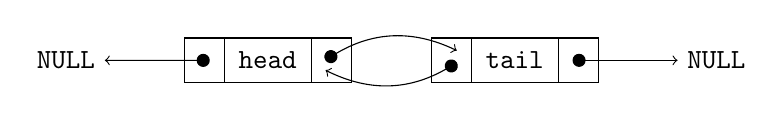
\begin{tikzpicture}[
      list/.style={
            rectangle split,
            rectangle split parts=3, draw,
            rectangle split horizontal,
            inner sep=5pt, text=black
        },
        ->, start chain
      ]
    \node[list,on chain] (A) {\nodepart{second} \texttt{head}};
    \node[list,on chain] (C) {\nodepart{second} \texttt{tail}};

    \node (D) [right=of C] {\texttt{NULL}};
    \node (E) [left= of A] {\texttt{NULL}};

    \path[*->] let \p1 = (A.three), \p2 = (A.center) in
    (\x1,\y2) edge [bend left] ($(C.one)+(0.15,0.2)$);

    \draw[*->] let \p1 = (C.three), \p2 = (C.center) in (\x1,\y2) -- (D);
    \draw[*->] ($(A.one)+(0.15,0.075)$) -- (E);

    \path[*->] ($(C.one)+(0.15,0.05)$) edge [bend left] ($(A.three)+(0,-0.05)$);
  \end{tikzpicture}
\end{center}

\begin{center}
  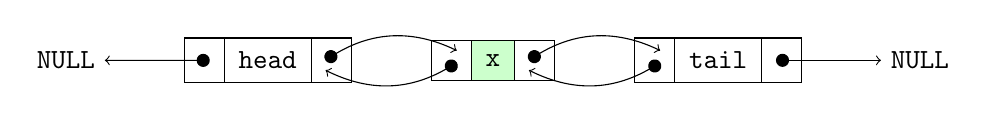
\begin{tikzpicture}[
      list/.style={
            rectangle split,
            rectangle split parts=3, draw,
            rectangle split horizontal,
            inner sep=5pt, text=black
        },
      new/.style={
            rectangle split,
            rectangle split parts=3, draw,
            rectangle split horizontal,
            inner sep=5pt, text=black,
            rectangle split part fill={white, green!20, white}
        },
      ->, start chain
      ]
    \node[list,on chain] (A) {\nodepart{second} \texttt{head}};
    \node[new,on chain] (B) {\nodepart{second} \texttt{x}};
    \node[list,on chain] (C) {\nodepart{second} \texttt{tail}};
    \node (D) [right=of C] {\texttt{NULL}};
    \node (E) [left= of A] {\texttt{NULL}};

    \path[*->] let \p1 = (A.three), \p2 = (A.center) in
    (\x1,\y2) edge [bend left] ($(B.one)+(0.15,0.2)$);

    \path[*->] let \p1 = (B.three), \p2 = (B.center) in
    (\x1,\y2) edge [bend left] ($(C.one)+(0.15,0.2)$);

    \draw[*->] let \p1 = (C.three), \p2 = (C.center) in (\x1,\y2) -- (D);

    \draw[*->] ($(A.one)+(0.15,0.075)$) -- (E);
    \path[*->] ($(B.one)+(0.15,0.05)$) edge [bend left] ($(A.three)+(0,-0.05)$);
    \path[*->] ($(C.one)+(0.15,0.05)$) edge [bend left] ($(B.three)+(0,-0.05)$);
  \end{tikzpicture}
\end{center}

\begin{center}
  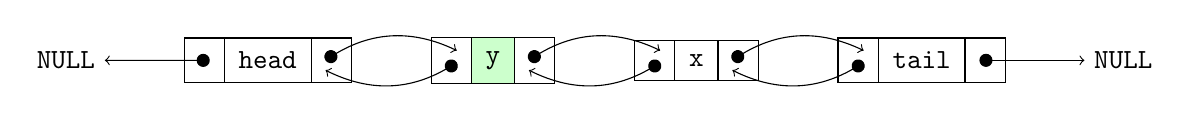
\begin{tikzpicture}[
      list/.style={
            rectangle split,
            rectangle split parts=3, draw,
            rectangle split horizontal,
            inner sep=5pt, text=black
        },
      new/.style={
            rectangle split,
            rectangle split parts=3, draw,
            rectangle split horizontal,
            inner sep=5pt, text=black,
            rectangle split part fill={white, green!20, white}
        },
      ->, start chain
      ]
    \node[list,on chain] (A) {\nodepart{second} \texttt{head}};
    \node[new,on chain] (F) {\nodepart{second} \texttt{y}};
    \node[list,on chain] (B) {\nodepart{second} \texttt{x}};
    \node[list,on chain] (C) {\nodepart{second} \texttt{tail}};
    \node (D) [right=of C] {\texttt{NULL}};
    \node (E) [left= of A] {\texttt{NULL}};

    \path[*->] let \p1 = (A.three), \p2 = (A.center) in
    (\x1,\y2) edge [bend left] ($(F.one)+(0.15,0.2)$);

    \path[*->] let \p1 = (F.three), \p2 = (F.center) in
    (\x1,\y2) edge [bend left] ($(B.one)+(0.15,0.2)$);

    \path[*->] let \p1 = (B.three), \p2 = (B.center) in
    (\x1,\y2) edge [bend left] ($(C.one)+(0.15,0.2)$);

    \draw[*->] let \p1 = (C.three), \p2 = (C.center) in (\x1,\y2) -- (D);

    \draw[*->] ($(A.one)+(0.15,0.075)$) -- (E);
    \path[*->] ($(F.one)+(0.15,0.05)$) edge [bend left] ($(A.three)+(0,-0.05)$);
    \path[*->] ($(B.one)+(0.15,0.05)$) edge [bend left] ($(F.three)+(0,-0.05)$);
    \path[*->] ($(C.one)+(0.15,0.05)$) edge [bend left] ($(B.three)+(0,-0.05)$);
  \end{tikzpicture}
\end{center}

\subsection{\texttt{void ll\_delete(LinkedList **ll)}}

The destructor for a linked list. Each node in the linked list should be
freed using \texttt{node\_delete()}. The pointer to the linked list
should be set to \texttt{NULL}.

\subsection{\texttt{uint32\_t ll\_length(LinkedList *ll)}}

Returns the length of the linked list, which is equivalent to the number
of nodes in the linked list, \emph{not} including the head and tail
sentinel nodes.

\subsection{\texttt{Node *ll\_lookup(LinkedList *ll, char
*oldspeak)}}

Searches for a node containing \texttt{oldspeak}. If a node is found,
the pointer to the node is returned. Else, a \texttt{NULL} pointer is
returned. If a node was found and the move-to-front option was specified
when constructing the linked list, then the found node is moved to the
front of the linked list. The move-to-front technique decreases look-up
times for nodes that are frequently searched for. You will learn more
about optimality in your future classes.

\subsection{\texttt{void ll\_insert(LinkedList *ll, char *oldspeak,
char *newspeak)}}

Inserts a new node containing the specified \texttt{oldspeak} and
\texttt{newspeak} into the linked list. Before inserting the node, a
look-up is performed to make sure the linked list \emph{does not} already
contain a node containing a matching \texttt{oldspeak}. If a duplicate
exists, a new node is not inserted into the linked list. Else, the new
node is inserted \emph{at the head} of the linked list. This means
that the new node comes directly after the head sentinel node.

\subsection{\texttt{void ll\_print(LinkedList *ll)}}

Prints out each node in the linked list \emph{except} for the head and
tail sentinel nodes. This will require the use of
\texttt{node\_print()}.

\vspace{10pt}
\begin{prelab}{Pre-lab Part 2}
  \begin{enumerate}
    \item Write down the pseudocode for each of the functions in the
      interface for the linked list ADT.
  \end{enumerate}
\end{prelab}


\section{Lexical Analysis with Regular Expressions}

\epigraph{\emph{Ideas are more powerful than guns. We would not let our
enemies have guns, why should we let them have ideas.}}{---Joseph
Stalin}

Back to regulating your citizens of the GPRSC. You will need a function
to parse out the words that they speak, which will be passed to you in
the form of an input stream. The words that they will use are valid
words, which can include \emph{contractions} and \emph{hyphenations}.
A valid word is any sequence of one or more characters that are part of
your regular expression word character set. Your word character set
should contain characters from $a-z$, $A-Z$, $0-9$, including the
underscore character. Since you also accept contractions like ``don't''
and ``y'all've'' and hyphenations like ``pseudo-code'' and
``move-to-front'', your word character set should include apostrophes
and hyphens as well.

You will need to write your own \emph{regular expression} for a word,
utilizing the \texttt{regex.h} library to lexically analyze the input
stream for words. You will be given a parsing module that lexically
analyzes the input stream using your regular expression. You are not
required to use the module itself, but it is \emph{mandatory} that you
parse through an input stream for words using at least one regular
expression. The interface for the parsing module will be in
\texttt{parser.h} and its implementation will be in \texttt{parser.c}.

The function \texttt{next\_word()} requires two inputs, the input stream
\texttt{infile}, and a pointer to a compiled regular expression,
\texttt{word\_regex}. Notice the word \emph{compiled}: you must first compile
your regular expression using \texttt{regcomp()} before passing it to the
function. Make sure you remember to call the function \texttt{clear\_words()} to
free any memory used by the module when you're done reading in words.
Here is a small program that prints out words input to \texttt{stdin}
using the parsing module. In the program, the regular expression for a
word matches one or more lowercase and uppercase letters. The regular
expression you will have to write for your assignment will be more
complex than the one displayed here, as it is just an example.

\begin{codelisting}{Example program using the parsing module.}
#include "parser.h"
#include <regex.h>
#include <stdio.h>

#define WORD "[a-zA-Z]+"

int main(void) {
    regex_t re;
    if (regcomp(&re, WORD, REG_EXTENDED)) {
        fprintf(stderr, "Failed to compile regex.\n");
        return 1;
    }

    char *word = NULL;
    while ((word = next_word(stdin, &re)) != NULL) {
        printf("Word: %s\n", word);
    }

    clear_words();
    regfree(&re);
    return 0;
}
\end{codelisting}

\vspace{10pt}
\begin{prelab}{Pre-lab Part 3}
  \begin{enumerate}
    \item Write down the regular expression you will use to match words
      with. It should match hyphenations and contractions as well. The
      regular expression refers to the pattern you will be using. For
      example, a regular expression to match strings consisting of only
      lowercase characters would be: \texttt{"[a-z]+"}.
  \end{enumerate}
\end{prelab}


\section{Your Task}

\epigraph{\emph{The people will believe what the media tells them they
believe.}}{---George Orwell}

\begin{itemize}
  \item Initialize your Bloom filter and hash table.
  \item Read in a list of \emph{badspeak} words with \texttt{fscanf()}.
    Again, badspeak is simply oldspeak without a newspeak translation.
    Badspeak is strictly forbidden. Each badspeak word should be added
    to the Bloom filter and the hash table. The list of proscribed words
    will be in \texttt{badspeak.txt}, which can be found in the
    \texttt{resources} repository.
  \item Read in a list of \emph{oldspeak} and \emph{newspeak} pairs with
    \texttt{fscanf()}. Only the oldspeak should be added to the Bloom
    filter. The oldspeak \emph{and} newspeak are added to the hash
    table. The list of oldspeak and newspeak pairs will be in
    \texttt{newspeak.txt}, which can also be found in the
    \texttt{resources} repository.
  \item Now that the lexicon of badspeak and oldspeak/newspeak
    translations has been populated, you can start to filter out words.
    Read words in from \texttt{stdin} using the supplied parsing module.
  \item For each word that is read in, check to see if it has been added
    to the Bloom filter. If it has not been added to the Bloom filter,
    then no action is needed since the word isn't a proscribed word.
  \item If the word has most likely been added to the Bloom filter,
    meaning \texttt{bf\_probe()} returned \texttt{true}, then further
    action needs to be taken.
    \begin{enumerate}
      \item If the hash table contains the word and the word \emph{does
        not} have a newspeak translation, then the citizen who used this
        word is guilty of \texttt{thoughtcrime}. Insert this badspeak
        word into a list of badspeak words that the citizen used in
        order to notify him of his errors later.
      \item If the hash table contains the word, and the word \emph{does}
        have a newspeak translation, then the citizen requires
        counseling on proper \emph{Rightspeak}. Insert this oldspeak
        word into a list of oldspeak words with newspeak translations in
        order to notify the citizen of the revisions needed to be made
        in order to practice Rightspeak.
      \item If the hash table does not contain the word, then all is
        good since the Bloom filter issued a false positive. No
        disciplinary action needs to be taken.
    \end{enumerate}
  \item If the citizen is accused of thoughtcrime \emph{and} requires
    counseling on proper \emph{Rightspeak}, then they are given a
    reprimanding message notifying them of their transgressions and
    promptly sent off to \emph{joycamp}. The message should both contain
    the list of badspeak words and oldspeak words with newspeak
    translations that were used.

    \begin{lstlisting}[style=plainstyle]
    Dear Comrade,

    You have chosen to use degenerate words that may cause hurt
    feelings or cause your comrades to think unpleasant thoughts.
    This is doubleplus bad. To correct your wrongthink and
    preserve community consensus we will be sending you to joycamp
    administered by Medellin's Miniluv. Beware of the hippos.

    Your errors:

    kalamazoo
    antidisestablishmentarianism

    Think of these words on your vacation!

    sad -> happy
    liberty -> badfree
    music -> noise
    read -> papertalk
    write -> papertalk\end{lstlisting}

  \item If the citizen is accused solely of thoughtcrime, then they are
    issued a thoughtcrime message and also set off to \emph{joycamp}.
    The message should contain the list of badspeak words that were
    used.

  \begin{lstlisting}[style=plainstyle]
  Dear Comrade,

  You have chosen to use degenerate words that may cause hurt
  feelings or cause your comrades to think unpleasant thoughts.
  This is doubleplus bad. To correct your wrongthink and
  preserve community consensus we will be sending you to joycamp
  administered by Medellin's Miniluv. Beware of the hippos.

  Your errors:

  kalamazoo
  antidisestablishmentarianism\end{lstlisting}

  \item If the citizen only requires counseling, then they are issued an
    encouraging \emph{goodspeak message}. They will read it, correct
    their \emph{wrongthink}, and enjoy the rest of their stay in the
    GPRSC. The message should contain the list of oldspeak words with
    newspeak translations that were used.

    \begin{lstlisting}[style=plainstyle]
    Dear Comrade,

    Submitting your text helps to preserve feelings and prevent
    badthink. Some of the words that you used are not goodspeak.
    The list shows how to turn the oldspeak words into newspeak.

    sad -> happy
    liberty -> badfree
    music -> noise
    read -> papertalk
    write -> papertalk\end{lstlisting}

  \item The list of the command-line options your program must support
    is listed below. \emph{Any} combination of the command-line options
    must be supported.
    \begin{itemize}
      \item \texttt{-h size} specifies that the hash table
        will have \texttt{size} entries (the default will be $10000$).
      \item \texttt{-f size} specifies that the Bloom filter
        will have \texttt{size} entries (the default will be $2^{20}$).
      \item \texttt{-m} will enable the \emph{move-to-front rule}.
    \end{itemize}
\end{itemize}


\section{Deliverables}

\epigraph{\emph{I would rather have questions that can't be answered than
answers that can't be questioned.}}{---Richard P. Feynman}

You will need to turn in:

\begin{enumerate}
  \item \texttt{banhammer.c}: This contains \texttt{main()} and
    \emph{may} contain the other functions necessary to complete the
    assignment.
  \item \texttt{speck.h}: Defines the interface for the hash function
    using the SPECK cipher. Do not modify this.
  \item \texttt{speck.c}: Contains the implementation of the hash
    function using the SPECK cipher. Do not modify this.
  \item \texttt{hash.h}: Defines the interface for the hash table ADT.
    Do not modify this.
  \item \texttt{hash.c}: Contains the implementation of the hash table
    ADT.
  \item \texttt{ll.h}: Defines the interface for the linked list ADT. Do
    not modify this.
  \item \texttt{ll.c}: Contains the implementation of the linked list
    ADT.
  \item \texttt{node.h}: Defines the interface for the node ADT. Do not
    modify this.
  \item \texttt{node.c}: Contains the implementation of the node ADT.
  \item \texttt{bf.h}: Defines the interface for the Bloom filter ADT.
    Do not modify this.
  \item \texttt{bf.c}: Contains the implementation of the Bloom filter ADT.
  \item \texttt{bv.h}: Defines the interface for the bit vector ADT. Do
    not modify this.
  \item \texttt{bv.c}: Contains the implementation of the bit vector
    ADT.
  \item \texttt{parser.h}: Defines the interface for the regex parsing
    module. Do not modify this.
  \item \texttt{parser.c}: Contains the implementation of the regex
    parsing module.
  \item You may have other source and header files, but \emph{do not
    make things overly complicated}.
  \item \texttt{Makefile}: This is a file that will allow the grader to
    type \texttt{make} to compile your program.
  \begin{itemize}
      \item \texttt{CFLAGS=-Wall -Wextra -Werror -Wpedantic}
        must be included.
      \item \texttt{CC=clang} must be specified.
      \item \texttt{make clean} must remove all files that are compiler
        generated.
      \item \texttt{make} should build your program, as should
        \texttt{make all}.
      \item Your program executable \emph{must} be named
        \texttt{banhammer}.
      \item Running \texttt{scan-build} on your program should result in
        no reported bugs. If there are any false positives that are
        reported, they should be explained in \texttt{README.md}.
  \end{itemize}

  \item \texttt{README.md}: This must be in Markdown. This must describe
    how to use your program and \texttt{Makefile}. This includes listing
    and explaining the command-line options that your program accepts.
    Any false positives reported by \texttt{scan-build} should go here
    as well.

  \item \texttt{DESIGN.pdf}: This \emph{must} be a PDF. The design
    document should contain answers to the pre-lab questions at the
    beginning and describe your design for your program with enough
    detail that a sufficiently knowledgeable programmer would be able to
    replicate your implementation.  This does not mean copying your
    entire program in verbatim. You should instead describe how your
    program works with supporting pseudo-code. For this program, pay
    extra attention to how you build each necessary component.

  \textcolor{red}{You \emph{must} push the \texttt{DESIGN.pdf} before
  you push \emph{any} code.}
\end{enumerate}


\section{Submission}

\epigraph{\emph{We can and must write in a language which sows among the
masses hate, revulsion, and scorn toward those who disagree with
us.}}{---Vladimir Lenin}

\noindent To submit your assignment, refer back to \texttt{assignment0}
for the steps on how to submit your assignment through \texttt{git}.
Remember: \emph{add, commit,} and \emph{push}!

\textcolor{red}{Your assignment is turned in \emph{only} after you have
  pushed and turned in the commit ID to Canvas. If you forget to push,
  you have not turned in your assignment and you will get a \emph{zero}.
  ``I forgot to push'' is not a valid excuse. It is \emph{highly}
  recommended to commit and push your changes \emph{often}.}


% \section{Supplemental Readings}

% \epigraph{\emph{The more you read, the more things you will know. The
% more that you learn, the more places you'll go.}}{---Dr.\ Seuss}\noindent

% \begin{itemize}
%   \item \textit{The C Programming Language} by Kernighan \& Ritchie
%   \begin{itemize}
%     \item Chapter 1 \S 1.5
%     \item Chapter 5 \S 5.6--5.12
%     \item Chapter 8 \S 8.1--8.3
%   \end{itemize}
% \end{itemize}

\end{document}

